\section{LLVM}

% TODO: update llvm information in references
\say{The LLVM Project is a collection of modular and reusable compiler and toolchain technologies. The LLVM project has multiple components. The core of the project is itself called “LLVM”. This contains all of the tools, libraries, and header files needed to process intermediate representations and converts it into object files. Tools include an assembler, disassembler, bitcode analyzer, and bitcode optimizer.} \cite{llvm,lattner2004llvm} LLVM takes an \textbf{intermediate representation (IR)} of a program, and translates it to machine language.

\begin{figure}[htpb]
    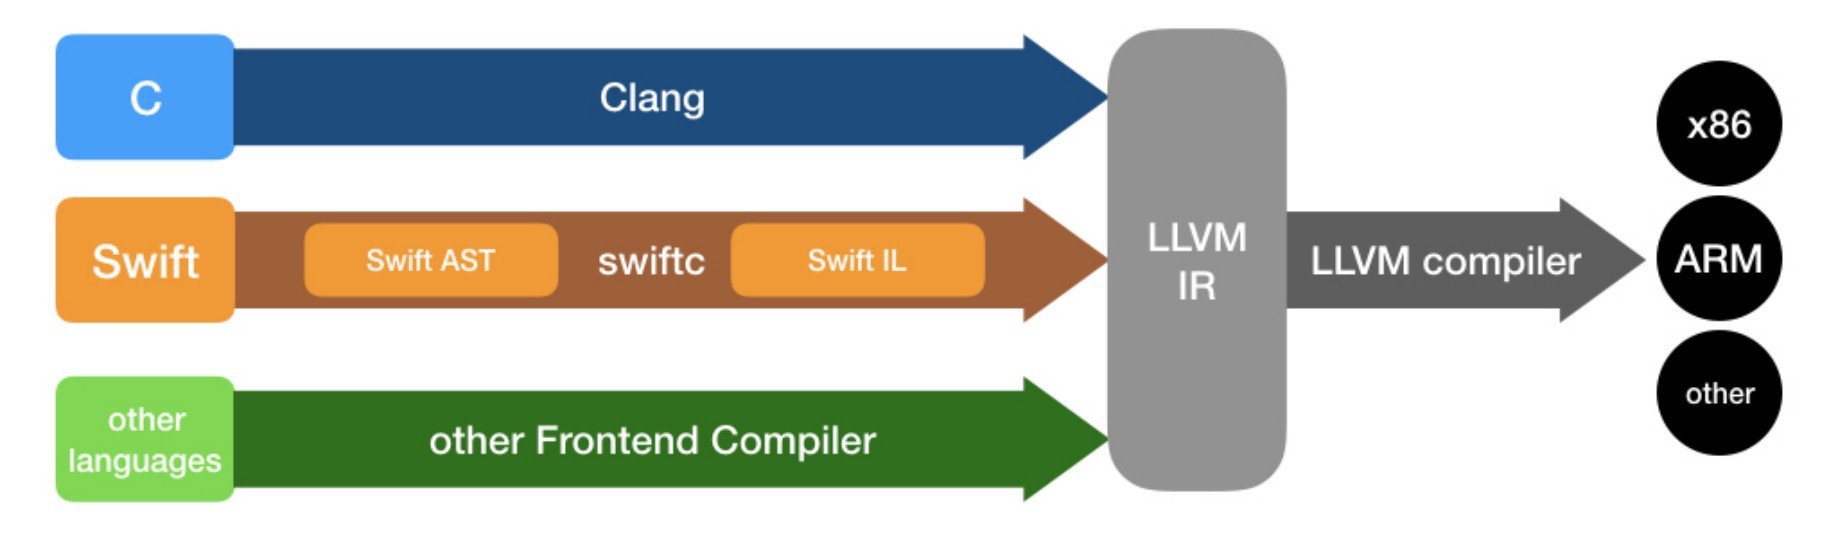
\includegraphics[width=\textwidth]{Chapter2/llvm.png}
    \centering
    \captionsetup{justification=centering}
    \caption{LLVM architecture: A front-end compiler generates the LLVM IR, and then it is converted into machine code \cite{omni_sci}}
    \label{fig:llvm}
\end{figure}

\say{\textbf{clang} is a C, C++, and Objective-C compiler which encompasses preprocessing, parsing, optimization, code generation, assembly, and linking.}\cite{clang} It parses the source code, using the language-specific syntax, and converts it into a language-agnostic IR. We can use this feature for our instrumentation as it is followed.

\newpage

\subsection{Instrumentation and coverage measurements}
\label{instrumentation}

The goal of using instrumentation for AFL, is to differentiate code coverages. AFL takes the source code and an instrumentation recipe, and generates the instrumented binary of the target program.

The recipe for instrumentation, fills out the coverage bitmap with the hash values of the path executed. The instructions are as followed:

\begin{lstlisting}[language=C++,style=CodeStyle]
  cur_location = <COMPILE_TIME_RANDOM>;
  shared_mem[cur_location ^ prev_location]++; 
  prev_location = cur_location >> 1;
\end{lstlisting}

AFL instruments by adding these instructions into basic blocks. First, a random value is assigned to \textit{curr\_location}. Next, it is XORed with the previous location's value, \textit{prev\_location}, and the resulting value is the location on \textit{shared\_mem}, the \textit{coverage bitmap}, which is incremented by one. The third and final instruction is reseting the \textit{prev\_location} to a new value.

When AFL runs the instrumented program, everytime an instrumented basic block is executed, a location of $shared\_mem$ in bitmap is increased. The reason for this algorithm is for differentiating different paths that go over the same basic blocks. For instance, in figure \ref{fig:instrumentation}, suppose that we have an instrumented program, with the random values set in compile time. A simple execution would be walking over basic blocks $1\rightarrow2\rightarrow5$ will increase these locations by 1: $shared\_mem[2362223]$ for the transition of $1\rightarrow2$ and $shared\_mem[368221416]$ for $2\rightarrow5$. We can see that the paths $1\rightarrow3\rightarrow4\rightarrow5$ and $1\rightarrow3\rightarrow4\rightarrow3\rightarrow4\rightarrow5$ (which contains a loop), set different values on bitmap.


\begin{figure}[htpb]
    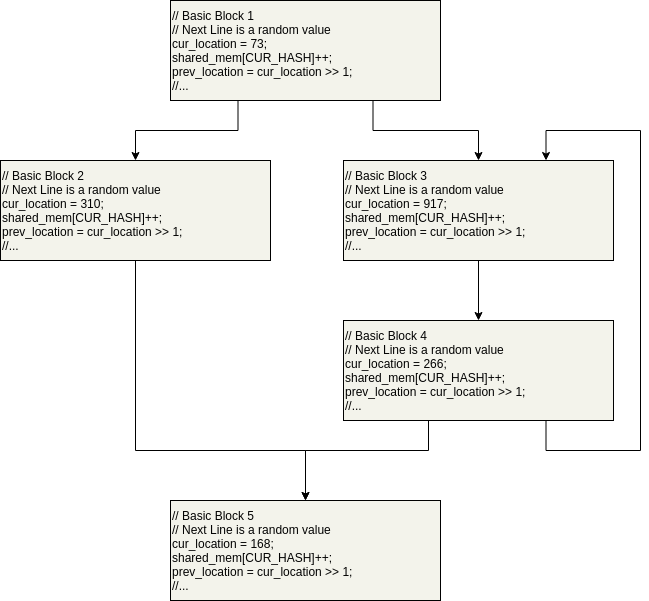
\includegraphics[width=\textwidth]{Chapter2/instrumentation.png}
    \centering
    \captionsetup{justification=centering}
    \caption{Example for instrumented basic blocks}
    \label{fig:instrumentation}
\end{figure}

AFL has the recipe for inserting the above instructions to the basic blocks using LLVM. It first compiles the program using this recipe for clang and after the execution of the program, we have a coverage bitmap of the locations we have visited during the execution. As a result, AFL uses this coverage feature for announcing new inputs with new coverages.
